\chapter{Portfolio extension: indicators and consequences}
\label{app:portfolio}

Section~\ref{sec:approach-selection} ranks a wall with the failure model where
one exists and with indicators where it does not, and combines either with a
consequence class in a $3\times3$ risk matrix. This appendix gives both scores.
It builds on the team's earlier scoring framework, which followed ARK
\parencite{ark2023} and combined traffic, land use, movement, maintenance and
age in one index. That index mixed indicators of the probability of failure
with indicators of its consequences, so the two sides are separated here.

\section{Probability side for walls without a model}\label{app:portfolio-hazard}

For the sheet pile walls, the concrete walls and the kademuren, which the
failure model of Section~\ref{sec:prob} does not describe, five indicators are
scored from 1 (low concern) to 5 (high concern) and weighted
(Table~\ref{tab:portfolio-indicators}). The score is proposed, not applied: the
condition and maintenance records are not public. Within each group of similar
walls, the third with the highest score gets a high probability class and the
lowest third a low one, so a wall is only ranked against walls with the same
mechanism. Poor data raise the score, so missing evidence leads to an
inspection rather than to a low class. Age has the smallest weight, as the
theoretical end of life is the rule the municipality wants to move away from
\parencite{utrecht_teamchallenge2026}, and Section~\ref{sec:regression} finds
height and age weak indicators on their own. The weights are assumptions, to be
tested once the records are available.

\begin{table}[htbp]
\centering
\small
\caption{Indicator score for walls without a failure model: weight and the
values that give scores 1 to 5.}
\label{tab:portfolio-indicators}
\begin{tabularx}{\textwidth}{@{}l r >{\raggedright\arraybackslash}X >{\raggedright\arraybackslash}p{3.4cm}@{}}
\toprule
Indicator & Weight & Scores 1 to 5 & Source \\
\midrule
Observed movement & 30\,\% & Vertical rate below 1, 1--2, 2--3, 3--5, above 5\,mm/yr & \textcite{bodemdalingskaart} \\
Condition & 30\,\% & NEN~2767 score 1--2, 3, 4, 5, 6 & Latest inspection \parencite{nen2767} \\
Maintenance history & 15\,\% & Last structural intervention within 10, 10--20, 20--30, 30--50 years, longer or unknown & Register, programme records \\
Data quality & 15\,\% & 1 drawings and a recent inspection, 3 register only, 4 rounded year, 5 missing or collective year & Register (Table~\ref{tab:data-quality}) \\
Age & 10\,\% & Below 50, 50--100, 100--150, 150--200, above 200 years & Register \\
\bottomrule
\end{tabularx}
\end{table}

\section{Consequence side}\label{app:portfolio-consequence}

Three indicators are scored from 1 (low) to 3 (high); the consequence class is
low for a mean below 1.75, high from 2.5, and medium in between:
\begin{itemize}
  \item \emph{People}: restaurants, cafes, bars and outdoor seating within
    20\,m of the wall in OpenStreetMap \parencite{osm2026}: below 0.5 per
    100\,m scores 1, from 3 per 100\,m scores 3. Outside the werven, land use
    takes its place.
  \item \emph{Cellars}: the share of the wall with the front of a wharf cellar
    within 15\,m in the municipal Werfmuren layer \parencite{utrecht_werfmuren}:
    below 0.25 scores 1, from 0.75 scores 3. Outside the werven, buildings
    within the failure zone take its place.
  \item \emph{Reachability}: the distance from the wall to the street behind
    the werf in the BGT \parencite{bgt}: closer than 3\,m scores 3, farther than
    6\,m scores 1. For walls along roads, traffic intensity takes its place.
\end{itemize}
Cables, pipes and trees in the werf are not in open data and are left out;
heritage value is the same for every walmuur (national monument) and is not
scored.

\section{Application to the walmuren}\label{app:portfolio-walmuren}

The script \texttt{build\_walmuur\_consequence.py} scores the 51 walmuren and
\texttt{plot\_results\_map.py} combines the score with the failure probability
of the 17 modelled walls (Table~\ref{tab:risk-classes},
Figure~\ref{fig:results-map}). The probability class is relative: high if
$P_f$ exceeds 1.5 times the median of the modelled walls (0.146, $\beta$ 1.05),
low if it is below the median divided by 1.5. The sum of the two class scores
gives the risk class: 5 or 6 red, 4 orange, 2 or 3 green. The list is ordered
by risk class and, within a class, by $P_f$.

The relative class always marks some walls high, whatever their absolute
safety, and adding or removing walls can change the class of others. The
factor 1.5 is a choice: with 1.25, ten walls (466\,m) are red, two orange and
five green; with 2.0, six (361\,m) are red, nine orange and two green. Walls
whose prior chance of type~2 is 0.5, Kromme Nieuwe Gracht 005 to 009, have no
dive note on the wall type, and Appendix~\ref{app:prob-checks} shows that
their $\beta$ rests partly on the miscalibrated type-1 model; for them the class
signals missing data, and establishing the wall type comes before any other
measure.

Nearly every walmuur has cellars behind it, so that indicator separates
little; the walls differ mainly in the people on the werf, high on the
Oudegracht and low on the Kromme Nieuwegracht, and in the distance to the
street, short on the Kromme Nieuwegracht. Nine walls (398\,m) are red, three
(154\,m) orange and five (59\,m) green. As the walls are renewed around 2031,
the classes mainly set the order and the interim measures: red walls first,
with restricted use and a survey of the wall type.

\begin{figure}[htbp]
\centering
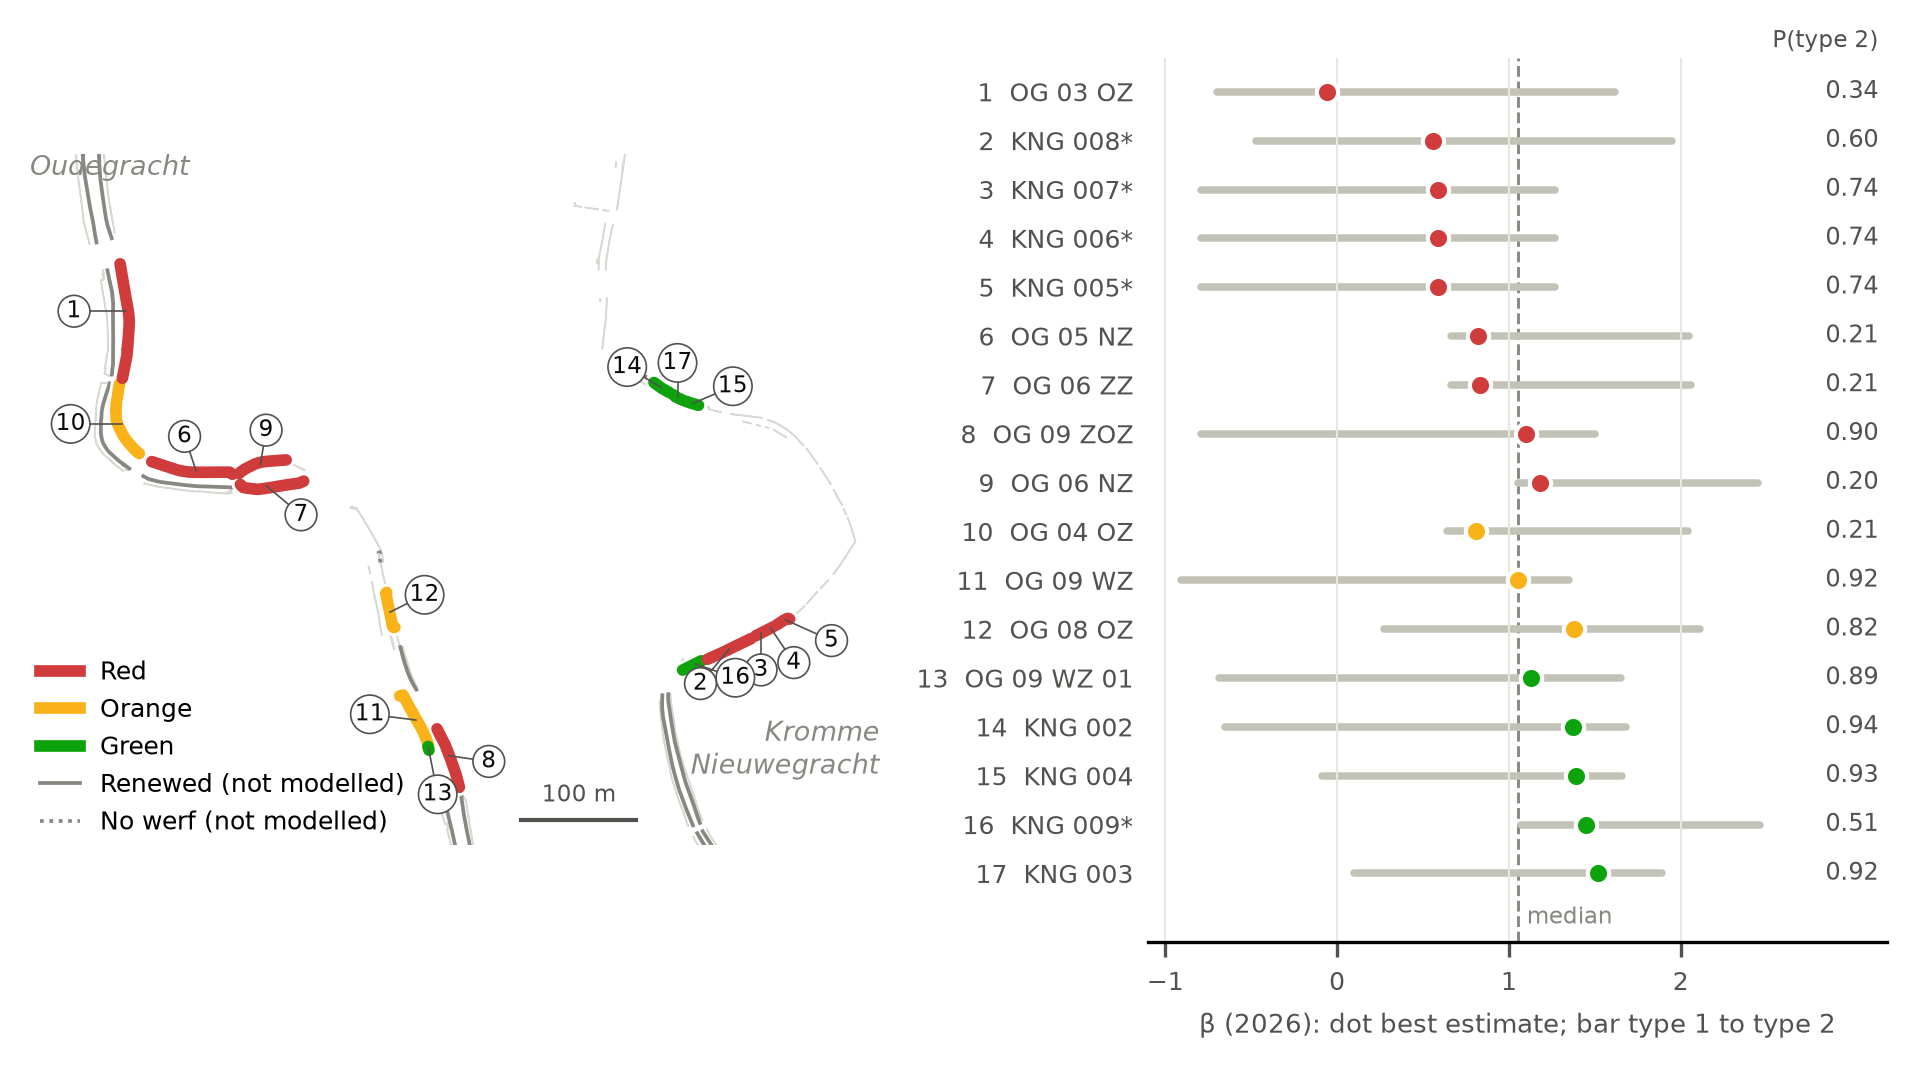
\includegraphics[width=\textwidth]{figures/results_map.png}
\caption{Risk class and $\beta$ of the 17 modelled walmuren. Right: best estimate of
$\beta$ (dot) and the range from type~1 to type~2 (bar), with the updated
probability of type~2; *: no dive note on the wall type, so the class rests on
missing data.}
\label{fig:app-results-beta}
\end{figure}

\begin{table}[htbp]
\centering
\small
\caption{Risk class of the 17 modelled walmuren. Hosp.: restaurants, cafes,
bars and outdoor seating per 100\,m; cellar: share of the wall with a cellar
front within 15\,m; road: distance to the street; scores for people, cellars
and reachability. OG = Oude Gracht, KNG = Kromme Nieuwe Gracht. *: no dive note
on the wall type; the class rests on missing data.}
\label{tab:risk-classes}
\setlength{\tabcolsep}{4pt}
\begin{tabular}{@{}r l r l r r r c l l@{}}
\toprule
 & Wall & $\beta$ & $P$ class & Hosp. & Cellar & Road [m] & Scores & Consequence & Risk \\
\midrule
1 & OG Rak 03 OZ & \textminus0.06 & high & 4.2 & 1.00 & 4.5 & 3/3/2 & high & red \\
2 & KNG 008* & 0.56 & high & 0.0 & 1.00 & 1.6 & 1/3/3 & medium & red \\
3 & KNG 007* & 0.59 & high & 0.0 & 1.00 & 1.7 & 1/3/3 & medium & red \\
4 & KNG 006* & 0.59 & high & 0.0 & 1.00 & 1.6 & 1/3/3 & medium & red \\
5 & KNG 005* & 0.59 & high & 0.0 & 1.00 & 2.8 & 1/3/3 & medium & red \\
6 & OG Rak 05 NZ & 0.82 & medium & 10.7 & 1.00 & 4.0 & 3/3/2 & high & red \\
7 & OG Rak 06 ZZ & 0.83 & medium & 4.1 & 1.00 & 3.6 & 3/3/2 & high & red \\
8 & OG Rak 09 ZOZ & 1.10 & medium & 8.5 & 1.00 & 4.3 & 3/3/2 & high & red \\
9 & OG Rak 06 NZ & 1.18 & medium & 4.8 & 1.00 & 3.1 & 3/3/2 & high & red \\
10 & OG Rak 04 OZ & 0.81 & medium & 10.2 & 1.00 & 6.7 & 3/3/1 & medium & orange \\
11 & OG Rak 09 WZ & 1.05 & medium & 6.4 & 0.39 & 13.2 & 3/2/1 & medium & orange \\
12 & OG Rak 08 OZ & 1.38 & low & 9.6 & 1.00 & 2.8 & 3/3/3 & high & orange \\
13 & OG Rak 09 WZ 01 & 1.13 & medium & 0.0 & 0.00 & 15.2 & 1/1/1 & low & green \\
14 & KNG 002 & 1.37 & low & 0.0 & 1.00 & 2.6 & 1/3/3 & medium & green \\
15 & KNG 004 & 1.39 & low & 2.0 & 1.00 & 3.2 & 2/3/2 & medium & green \\
16 & KNG 009* & 1.45 & low & 0.0 & 1.00 & 5.5 & 1/3/2 & medium & green \\
17 & KNG 003 & 1.52 & low & 2.0 & 1.00 & 4.6 & 2/3/2 & medium & green \\
\bottomrule
\end{tabular}
\end{table}
